\documentclass{article}
\usepackage{amsmath}
\usepackage{graphicx}
\usepackage{listings}

\begin{document}

\section*{PROBLEM STATEMENT}
To implement the Mid-Point Circle Drawing Algorithm in C using OpenGL, and to draw a circle with a given center and radius on a 2D plane. The program will also draw the coordinate axes to visualize the circle in the context of a Cartesian coordinate system.

\section*{THEORY}
The Mid-Point Circle Drawing Algorithm is an efficient way to draw a circle by determining the points of the circle using a decision parameter. It takes advantage of the circle's symmetry to reduce the number of points needed to be calculated. 

The algorithm starts at the top of the circle and works its way down to the x-axis, deciding at each step whether to move horizontally or diagonally to the next point based on the decision parameter. By calculating only one-eighth of the circle, it uses symmetry to plot the remaining points.

\section*{ALGORITHM}
\begin{enumerate}
    \item \textbf{Initialize}:
    \begin{itemize}
        \item Start with the initial point $(x, y) = (0, \text{radius})$.
        \item Calculate the initial decision parameter: $p = 1 - \text{radius}$.
    \end{itemize}
    \item \textbf{Plotting}:
    \begin{itemize}
        \item Plot the initial point and its symmetrical points.
        \item For each x from 0 to y:
        \begin{itemize}
            \item Increment x by 1.
            \item If $p < 0$:
            \begin{itemize}
                \item $p = p + 2x + 1$
            \end{itemize}
            \item Else:
            \begin{itemize}
                \item Decrement y by 1.
                \item $p = p + 2(x - y) + 1$
            \end{itemize}
            \item Plot the new point and its symmetrical points.
        \end{itemize}
    \end{itemize}
    \item \textbf{Termination}:
    \begin{itemize}
        \item The loop terminates when x equals y.
    \end{itemize}
\end{enumerate}

\section*{FLOWCHART}
\begin{center}
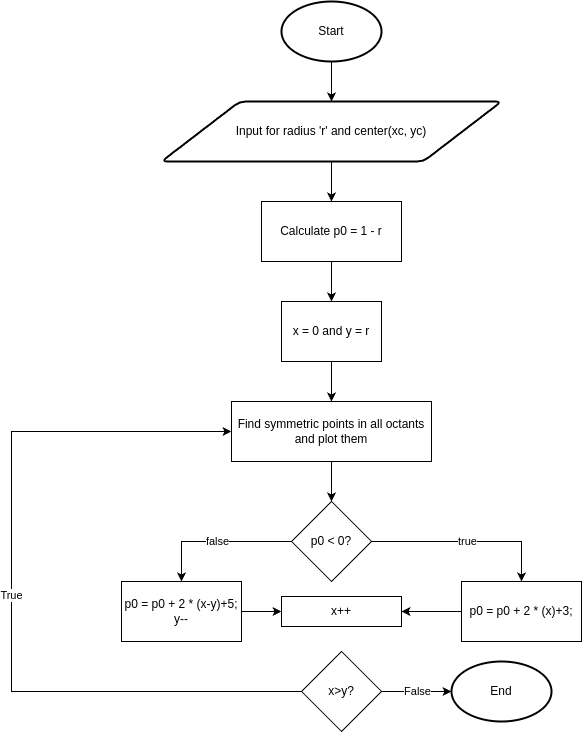
\includegraphics[width=0.7\textwidth]{flowchart.png}
\end{center}

\section*{SAMPLE I/O}
\textbf{Input:}
\begin{verbatim}
Enter the coordinates of the center of the circle (xc, yc): 0 0
Enter the radius of the circle: 50
\end{verbatim}

\textbf{Output:}
A circle is drawn with center $(0, 0)$ and radius $50$ on a window with coordinate axes displayed.

\section*{DISCUSSIONS}
\begin{itemize}
    \item \textbf{Accuracy}: The Mid-Point Circle Drawing Algorithm provides accurate and visually symmetric circles by efficiently calculating points based on the circle's symmetry.
    \item \textbf{Efficiency}: The algorithm is efficient due to its use of integer arithmetic and symmetry, reducing the number of calculations needed.
    \item \textbf{Applications}: The Mid-Point Circle Drawing Algorithm is used in various applications where circle drawing is required, such as computer graphics, game development, and CAD software.
\end{itemize}

\section*{CONCLUSION}
The Mid-Point Circle Drawing Algorithm is an effective method for rendering circles on raster displays. By calculating points based on the decision parameter and using symmetry, the algorithm ensures accurate and visually symmetric circles. The implementation using OpenGL demonstrates the algorithm's capability to draw circles with any given center and radius and visualize the coordinate axes.

\end{document}
